\subsubsection{Primera interacción con la aplicación dentro de la sala de clases}

{\textbf {Resumen:}}
El usuario (alumno enseñanza media) luego de que su profesor le hiciera entrega de una guía con la imagen QR de uno de los museos, descarga la aplicación indicada en esta, al terminar de descargar la app, la inicia, activa la cámara y apunta a la imagen con ella, al hacer esto el usuario visualiza sobre la imagen como se dibuja la habitación de un museo y ve en las indicaciones en pantalla, este se da cuenta de que puede explorar en la habitación para encontrar las piezas que esté muestra las cuales están escondidas dentro de este entorno. Además prueba las diferentes acciones para desplazarse por el museo. Luego al encontrar una pieza el usuario presiona sobre ella y descubre que ha encontrado un objeto, el cual es añadido a su colección de piezas, el usuario entusiasmado voltea a mostrarle a sus compañeros el descubrimiento.

{\textbf {Actores:}}
Alumno enseñanza media, Profesor.

{\textbf {Propósito:}}
Introducir al alumno el aprendizaje del museo local en cuestión, el cual se encuentra presente en la guía entregada por el profesor.

{\textbf {Tipo:}}
Primario.

{\textbf {Referencias cruzadas:}}
R 1.1, R 1.2, R 1.3, R 2.1, R 2.2, R 2.7, R 3.4, R 5.9.

\paragraph{Caso de Uso Esencial}

\begin{longtable}{|p{5cm}|p{8cm}|}
\hline 
Acción actores & Respuesta del sistema \\ 
\hline 
El profesor entrega al alumno el código QR & --- \\ 
\hline
El alumnos descarga la aplicación & Se muestran las indicaciones del uso necesario de la cámara \\ 
\hline 
El alumno enciende la cámara  & Se muestran las indicaciones de cómo interactúa con el código QR \\ 
\hline
El alumno apunta el código QR con su cámara & La aplicación detecta el código y carga un modelo 3d correspondiente al museo ligado a ese código.
Se le presentan las instrucciones de desplazamiento en el museo y se le informa que puede encontrar las piezas, del museo si las busca.
 \\ 
\hline
El alumno prueba las instrucciones de desplazamiento. & La aplicación cambia el escenario mostrado de acuerdo a las acciones hechas por el usuario. \\ 
\hline
El jugador ve una pieza y la presiona. & El sistema muestra una animación que confirma el haber encontrado la pieza y muestra una panel con información más detallada de esta \\ 
\hline
El alumno se voltea a mostrar su descubrimiento a su compañero. & --- \\ 
\hline
\caption{Tabla de Caso de Uso Esencial 1.1}
\label{tab21}
\end{longtable}

\paragraph{Diagrama de Caso de Uso}

\begin{figure}[H]
\centerline{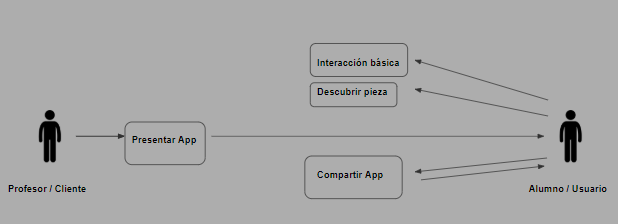
\includegraphics[width=15cm]{imgs/CasoUso_1.PNG}}
\caption{Diagrama de Caso 1.1}
\label{fig_1}
\end{figure}

\paragraph{Modelo Conceptual}

\begin{figure}[H]
\centerline{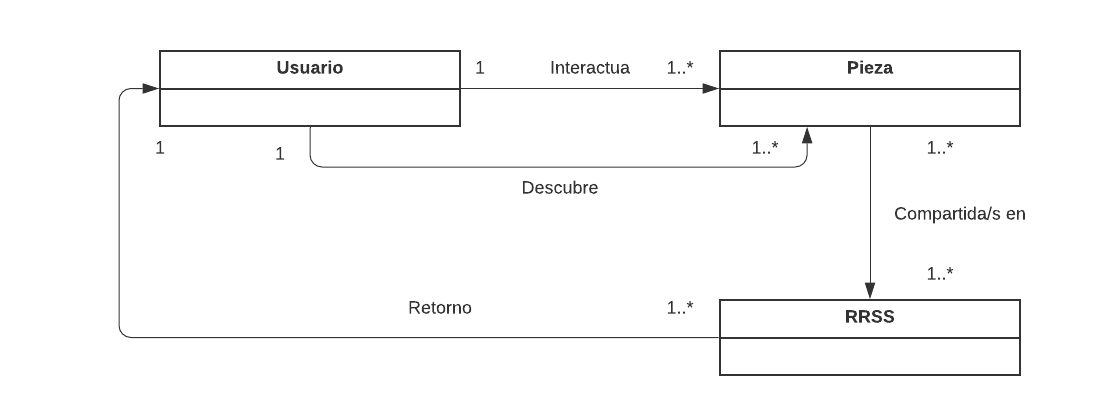
\includegraphics[width=15cm]{imgs/ModeloConceptualCaso_1_3.png}}
\caption{Modelo Conceptual Caso 1.1}
\label{fig_1_2}
\end{figure}

\paragraph{Diagrama de Secuencia o Colaboración}

\begin{figure}[H]
\centerline{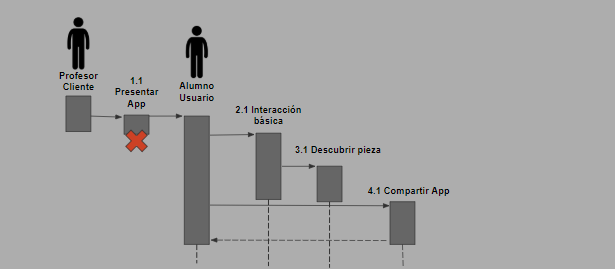
\includegraphics[width=15cm]{imgs/CasoUso_1_2.PNG}}
\caption{Diagrama de Secuencia Caso 1.1}
\label{fig_1_3}
\end{figure}

\subsubsection{Priorización}
{\textbf {Tipo:}}
Primario.